%% 
%% Copyright 2007-2020 Elsevier Ltd
%% 
%% This file is part of the 'Elsarticle Bundle'.
%% ---------------------------------------------
%% 
%% It may be distributed under the conditions of the LaTeX Project Public
%% License, either version 1.2 of this license or (at your option) any
%% later version.  The latest version of this license is in
%%    http://www.latex-project.org/lppl.txt
%% and version 1.2 or later is part of all distributions of LaTeX
%% version 1999/12/01 or later.
%% 
%% The list of all files belonging to the 'Elsarticle Bundle' is
%% given in the file `manifest.txt'.
%% 
%% Template article for Elsevier's document class `elsarticle'
%% with harvard style bibliographic references

\documentclass[authoryear,manuscript,12pt]{elsarticle}
\usepackage{setspace}
\doublespacing

\usepackage{algorithm}
\usepackage{algpseudocode}
\usepackage{rotating}
\usepackage{multirow}
\newtheorem{theorem}{Theorem}
\newtheorem{corollary}{Corollary}[theorem]
\newtheorem{lemma}[theorem]{Lemma}

\usepackage{xcolor}
\usepackage{tikz}
\usetikzlibrary{shapes.geometric,shapes.misc,shapes.symbols,arrows.meta,graphs,fit,positioning,shadows}

%% The `ecrc' package must be called to make the CRC functionality available
%\usepackage{ecrc}

%% Use the option review to obtain double line spacing
%% \documentclass[authoryear,preprint,review,12pt]{elsarticle}

%% Use the options 1p,twocolumn; 3p; 3p,twocolumn; 5p; or 5p,twocolumn
%% for a journal layout:
%% \documentclass[final,1p,times,authoryear]{elsarticle}
%% \documentclass[final,1p,times,twocolumn,authoryear]{elsarticle}
%% \documentclass[final,3p,times,authoryear]{elsarticle}
%% \documentclass[final,3p,times,twocolumn,authoryear]{elsarticle}
%% \documentclass[final,5p,times,authoryear]{elsarticle}
%% \documentclass[final,5p,times,twocolumn,authoryear]{elsarticle}

%% For including figures, graphicx.sty has been loaded in
%% elsarticle.cls. If you prefer to use the old commands
%% please give \usepackage{epsfig}

%% The amssymb package provides various useful mathematical symbols
\usepackage{amssymb}
%% The amsthm package provides extended theorem environments
%% \usepackage{amsthm}

%% The lineno packages adds line numbers. Start line numbering with
%% \begin{linenumbers}, end it with \end{linenumbers}. Or switch it on
%% for the whole article with \linenumbers.
%% \usepackage{lineno}

\journal{Computers \& Industrial Engineering}

\begin{document}

\begin{frontmatter}
%% Title, authors and addresses

%% use the tnoteref command within \title for footnotes;
%% use the tnotetext command for theassociated footnote;
%% use the fnref command within \author or \affiliation for footnotes;
%% use the fntext command for theassociated footnote;
%% use the corref command within \author for corresponding author footnotes;
%% use the cortext command for theassociated footnote;
%% use the ead command for the email address,
%% and the form \ead[url] for the home page:
%% \title{Title\tnoteref{label1}}
%% \tnotetext[label1]{}
%% \author{Name\corref{cor1}\fnref{label2}}
%% \ead{email address}
%% \ead[url]{home page}
%% \fntext[label2]{}
%% \cortext[cor1]{}
%% \affiliation{organization={},
%%            addressline={}, 
%%            city={},
%%            postcode={}, 
%%            state={},
%%            country={}}
%% \fntext[label3]{}

\title{Multi-product Batch Processing Time Maximization Problem}

%% use optional labels to link authors explicitly to addresses:
%% \author[label1,label2]{}
%% \affiliation[label1]{organization={},
%%             addressline={},
%%             city={},
%%             postcode={},
%%             state={},
%%             country={}}
%%
%% \affiliation[label2]{organization={},
%%             addressline={},
%%             city={},
%%             postcode={},
%%             state={},
%%             country={}}

%\author{Tatiana Balbi Fraga, Ítalo Ruan Barbosa de Aquino and Regilda da Costa e Silva Menêzes}

\author{Tatiana Balbi Fraga\corref{cor1}\fnref{label1}}
\ead{tatiana.balbi@ufpe.br}
\cortext[cor1]{corresponding author}

\author{Ítalo Ruan Barbosa de Aquino\fnref{label1}}
\ead{italo_ruan_@hotmail.com}

\author{Regilda da Costa e Silva Menêzes\fnref{label1}}
\ead{regilda.smenezes@ufpe.br}

%\affiliation[label1]{
%			 organization={Centro Acadêmico do Agreste - Universidade Federal de Pernambuco},
%             addressline={Avenida Marielle Franco, Bairro Nova Caruaru},
%             city={Caruaru},
%             postcode={55014-900},
%             state={PE},
%             country={Brasil} }

\affiliation[label1]{
		   organization={Agreste Academic Center - Federal University of Pernambuco},%Department and Organization
           addressline={Avenida Marielle Franco, Nova Caruaru}, 
           city={Caruaru},
           postcode={55014-900}, 
           state={PE},
           country={Brazil}}

\begin{abstract}
In the plastic bag extrusion process, it is necessary to determine the optimal processing time for batches formed by different products, which are processed simultaneously by the same extruder, but with different processing rates. The batch processing time must be determined in order to meet a series of known constraints, such as the limitation for the quantity produced for each product and for the quantity produced for the set of all products in the same batch. In this paper we present this problem as a new combinatorial optimization problem named Multi-product Batch Processing Time Maximization (MBPTM) problem. We also present a mathematical model for the MBPTM problem and an analytical solution method with polynomial time complexity, which proved to be able to obtain optimal solutions for several benchmarks in a very short time, even for very large instances.
\end{abstract}
%%Graphical abstract
%\begin{graphicalabstract}
%\end{graphicalabstract}

%%Research highlights
\begin{highlights}
\item brief bibliographic review on multi-product batch problems;
\item Multi-product Batch Processing Time Maximization (MBPTM) problem definition;
\item linear integer programming model for the MBPTM problem;
\item exact optimization method for solving the MBPTM problem.
\end{highlights}

\begin{keyword}
multiproduct batch \sep processing time maximization \sep mathematical model \sep analytical solution \sep LINGO
\end{keyword}
\end{frontmatter}

%% \linenumbers

%% main text
\section{Introduction}
\label{sec:intro}

The term multi-product batch production is usually applied to designate an intermittent production system in which batches of different products and sizes are processed one at a time, sharing the same production facilities. A multi-product batch plant basically consists of one or more units, grouped into one or more stages, and possibly, intermediate storage locations. At each stage some distinct operations are performed and the batches are processed sequentially over the stages (serial batching). As stated by \cite{PetkovMaranas1998} the batch plant can operate under a single-product campaign (SPC) production mode, where all the batches of a given product are manufactured before production of the next product begins, or under mixed-product campaign (MPC) production modes where more batches are produced per unit time at the expense of increased changeover times and cleanup costs. Also the plant layout can take on different formats, such as: single unit, where all batches are processed at a single stage; serial flowshop plant, in which all products follow a linear flow through the production stages; parallel plants in which production units of the same type are arranged in parallel, forming each production stage \citep{MendezEtAll2000, ShiEtAll2017}; and networked processes, in which units are not arranged in lines, and the connection between the units may or may not exist so that the production paths in the flowshop network can be different for each product and the passing of previous batch can be possible so that the final sequence of the production at the last stage units can be different from the initial sequence \citep{KimEtAl1996}.

The scientific literature address many different problems related to such industrial enviroment, including the design, planning, sizing, scheduling and balancing problems. The multi-product batch plant design problem is concerned to obtain the configuration of the plant and the equipment that minimize the capital cost of all the equipment items needed to fulfill the production requirements (Ravemark and Rippin, 1998). The configuration of the plant basically consists of defining the number of stages, the number of units and their capacity per stage, and the capacity for intermediate storages, as well as the best factory layout. 

The multi-product batch planning problem is basically determining the needs of materials and resources based on known demands and demand forecasts. 

Since a single batch is processed at a time, it is necessary that the batches are dimensioned in such a way that the quantity produced of each product is sufficient to meet the demand during the period in which other batches are being processed \citep{Eilon1985}. This problem is named multi-product batch sizing. \cite{Eilon1985} gives a detailed explanation of the inadequacy of the use of the well-know EBQ (economic batch quantity) square-root formula for multi-product batch production and \cite{LiuEtAl2020} present a mixed-integer quadratic programming model and an exact optimization algorithm for a multi-stage multi-product s-batch sizing problem in a networked plant of a steel industry (Fig. \ref{fig:networkdPlantSteelIndustry}). 

\begin{figure}[h]
\label{fig:networkdPlantSteelIndustry}
\begin{center}
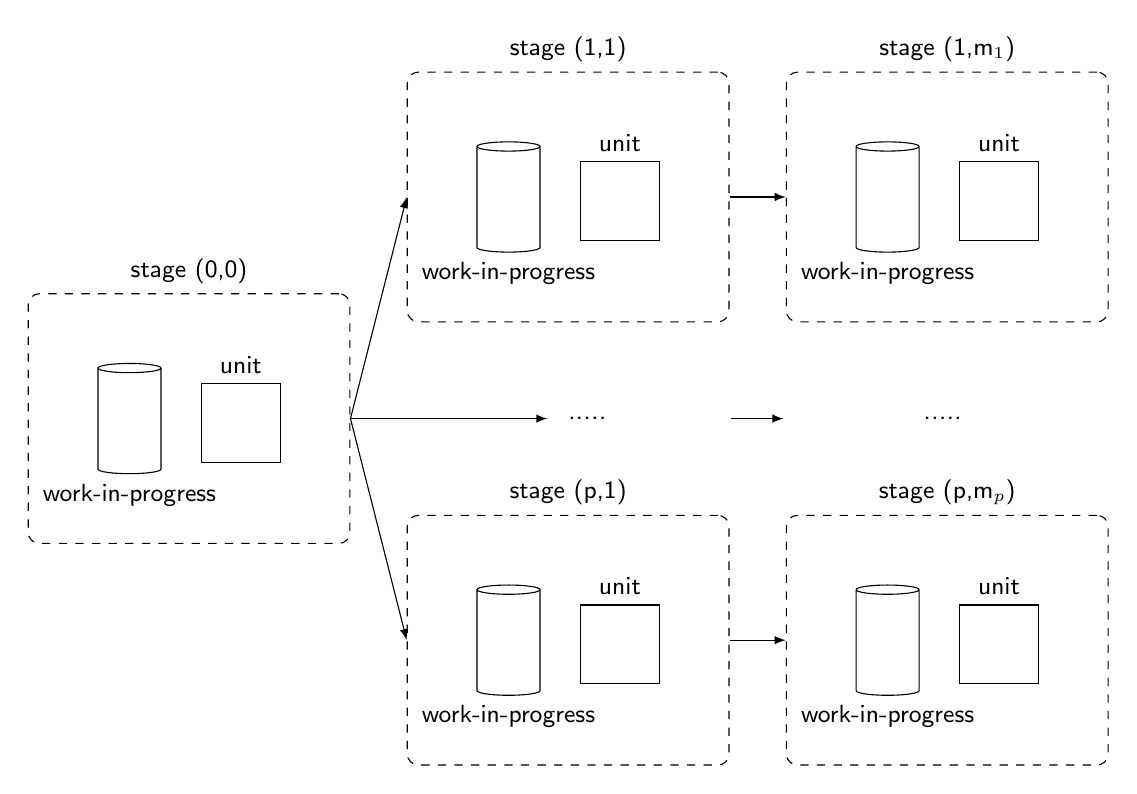
\begin{tikzpicture}[font=\sffamily,every label/.append style={font=\small\sffamily,align=center}]

\node[cylinder, cylinder uses custom fill, minimum width=0.8cm, minimum height=1.4cm, shape border rotate=90, aspect=0.5, draw, label={below:{work-in-progress}}](WIP00){};
\node[rectangle, draw, right=0.5cm of WIP00, minimum width=1cm, minimum height=1cm, label={above:{unit}}](unit00){};
\node[draw,dashed,rounded corners,fit=(WIP00) (unit00),inner sep=25pt,label={above:{stage (0,0)}}](stage00){};

\node[above right=2cm and 4cm of WIP00, cylinder, cylinder uses custom fill, minimum width=0.8cm, minimum height=1.4cm, shape border rotate=90, aspect=0.5, draw, label={below:{work-in-progress}}](WIP11){};
\node[rectangle, draw, right=0.5cm of WIP11, minimum width=1cm, minimum height=1cm, label={above:{unit}}](unit11){};
\node[draw,dashed,rounded corners,fit=(WIP11) (unit11),inner sep=25pt,label={above:{stage (1,1)}}](stage11){};

\draw[-latex] (stage00.east) -- (stage11.west);

\node[right=2.5cm of stage00, minimum width=1cm, minimum height=1.4cm](WIP1){.....};

\node[right=0.3cm of WIP1, minimum width=1cm, minimum height=1.4cm](WIP1a){};

\draw[-latex] (stage00.east) -- (WIP1.west);

\node[below right=2cm and 4cm of WIP00, cylinder, cylinder uses custom fill, minimum width=0.8cm, minimum height=1.4cm, shape border rotate=90, aspect=0.5, draw, label={below:{work-in-progress}}](WIPp1){};
\node[rectangle, draw, right=0.5cm of WIPp1, minimum width=1cm, minimum height=1cm, label={above:{unit}}](unitp1){};
\node[draw,dashed,rounded corners,fit=(WIPp1) (unitp1),inner sep=25pt,label={above:{stage (p,1)}}](stagep1){};

\draw[-latex] (stage00.east) -- (stagep1.west);

\node[right=4cm of WIP11, cylinder, cylinder uses custom fill, minimum width=0.8cm, minimum height=1.4cm, shape border rotate=90, aspect=0.5, draw, label={below:{work-in-progress}}](WIP1m){};
\node[rectangle, draw, right=0.5cm of WIP1m, minimum width=1cm, minimum height=1cm, label={above:{unit}}](unit1m){};
\node[draw,dashed,rounded corners,fit=(WIP1m) (unit1m),inner sep=25pt,label={above:{stage (1,m$_1$)}}](stage1m){};

\draw[-latex] (stage11.east) -- (stage1m.west);

\node[right=4cm of WIPp1, cylinder, cylinder uses custom fill, minimum width=0.8cm, minimum height=1.4cm, shape border rotate=90, aspect=0.5, draw, label={below:{work-in-progress}}](WIPpm){};
\node[rectangle, draw, right=0.5cm of WIPpm, minimum width=1cm, minimum height=1cm, label={above:{unit}}](unitpm){};
\node[draw,dashed,rounded corners,fit=(WIPpm) (unitpm),inner sep=25pt,label={above:{stage (p,m$_p$)}}](stagepm){};

\draw[-latex] (stagep1.east) -- (stagepm.west);

\node[right=3.5cm of WIP1, minimum width=1cm, minimum height=1.4cm](WIPm){.....};

\node[left=0.5cm of WIPm, minimum width=1cm, minimum height=1.4cm](WIPma){};

\draw[-latex] (WIP1a.east) -- (WIPma.west);

\end{tikzpicture}
\end{center}
\caption{Multi-product s-batch networked plant of a steel industry. Source: adapted from \cite{LiuEtAl2020} * stage $(i, j)$ means stage $j$ of production line $i$.}
\end{figure}

In multi-product batch scheduling (MPBS) problems it is necessary to determine the ideal batch size for each product and also the production sequence of the products batches based on the known demand. Here, the solution must be determined in such a way that both setup and storage costs are minimized \citep{Eilon1985, Omega1993, LiuEtAl2020}. Some cientific works impose additional constraints on the MPBS problem - such as release times and due dates for each products batch production, and sequencing constraints due to mismatched product colors sequences - and focus on other goals - such as optimize customer satisfaction and/or the plant performance \citep{MendezEtAll2000, ShiEtAll2017}. Also, some cientific works consider MPBS problems within different layouts and multiperiod scenario. In parallel MPBS as well as in networked processes, it can also be necessary to define in which units each batch will be processed, and constraints that limit the units that can process each batch can also be imposed.

It is importante to note that some production units are capable of processing multiple jobs at the same time. In such a case batches of different products and sizes can be grouped and processed by these units as a single batch. It is therefore necessary to determine the set of "batches" that each new grouped batch will contain. The multi-product balancing problem consists of determining these groupings, seeking to minimize the overall makespan. \cite{KashanOzturk2022} name this problem \emph{p-batch} (parallel batching) in contradiction with the \emph{s-batch} (serial batching) problem where jobs are processed one by one over production facilities, as described before.

In a real production environment, some of these problems arise in a connected way, so many cientific works adress mixed multi-product batch problems. \cite{FumeroEtAl2016} developed a multi-period mixed-integer linear programming model for MPCs multistage multi-product batch problems, which integrates design, production planning, and scheduling decisions. 

\cite{LiEtAl2022} deal with a PMPBS problem involving incompatible families with different job sizes and capacity constraints. In this problem, solutions are accepted in which two or more batches are processed simultaneously on the same machine. However, there are no production limitations for the production of each product group. The paper of \cite{LiEtAl2022} also presente an extensive literature review on production batch scheduling problems. Other important works deal with the problem of a multi-product batch plant design (MPBPD). In this case the problem is to obtain the configuration of the plant and the equipment that minimize the capital cost of all the equipment items needed to fulfill the production requirements (Ravemark and Rippin, 1998).

\begin{sidewaystable}[h]
\begin{center}
\begin{small}
\begin{tabular}[c]{|c|c|c|c|c|c|c|c|c|}
reference & problem & period & stage & units & int. stor. & constraints & objectives & method \\
\hline
\multirow{2}{*}{\cite{Eilon1985}} & \multirow{2}{*}{scheduling} & \multirow{2}{*}{single} & \multirow{2}{*}{single} & \multirow{2}{*}{single} & & & minimize total setup;  \\
 & & & & & & & minimize daily holding cost;  \\
\multirow{3}{*}{\cite{ShiEtAll2017}} & \multirow{3}{*}{scheduling} & \multirow{3}{*}{single} & non-identical & \multirow{3}{*}{unlimited} & release time \\
 & & & & parallel & & due date \\
 & & & & & \\
 & & & & \\
\end{tabular}
\label{tab:MBPTax}
\caption{Multi-product batch problems taxonomy}
\end{small}
\end{center}
\end{sidewaystable}

About the solution method many papers propose mathmatical models which are solved using IBM ILOG CPLEX or another constraint programming solver.

In this work we are interested in a sub problem of the \emph{p-batch} scheduling problem described by \cite{KashanOzturk2022}, named multi-product batch processing time maximization (MBPTM) problem. When appliyng some local search heuristic for solving the \emph{p-batch} scheduling problem it is necessary to solve the MBPTM problem on each iteration, so it has a direct impact on the overall efficiency of any local search heuristc for solving the \emph{p-batch} scheduling problem. As scientific contributions, in this paper we present a mathematical model and a polynomial time complexity optmization method for solving this problem.

The rest of the paper is organized as follows. In the next sections, a presentation of problem is made along with an application example. Section \ref{sec:mathModel} presents an interger linear mathematical model for the problem and section \ref{sec:analyticalSol} presents an analytical method for its solution. Section \ref{sec:results} presents the tests and results obtained by a solver in C++ applying the analytical solution and a solver developed in LINGO to new proposed benchmarks. In sections \ref{sec:contributions} and \ref{sec:acknowledgments}, the contributions to this work are informed and acknowledgments are given, respectively. Finally, section \ref{sec:conclusions} presents the paper's conclusions and suggestions for future works.

\section{Multi-product batch processing time maximization problem}
\label{sec:MBPTMP}

The multi-product batch processing time maximization problem arises when a set of different products are processed simultaneously in a same production batch. In this problem, it is considered that the quantity produced of each product is directly proportional to the processing time, however, with a different constant of proportionality (production rate) for each product. In addition, there is a maximum quantity allowed for the production of batch products, defined both individually and for the set. The production quantity of each product is mainly defined according to the demand for the product. However, it is still possible to stock the products and/or send them to the outlets. In both cases, there is a stocking/shipping limit for each product and a stocking/shipping limit for the set of products in the batch. Also, there is a time limit available for processing the batch. About the production, the industry manager has as priority to meet demand and he prefer to send the remaining production to outlets rather then stock it in the factory. 

\emph{Example:} A certain machine must process a batch containing 2 different products: A and B. The production rate of A is 60 g/min while the production rate of B is 40 g/min. The factory has free stock for a maximum of 3000 g of any product, and, according to the company's inventory policy, a maximum of 3000 g of product A and 2000 g of product B can be stocked at the factory. There is a demand for 1000 g of product A and 500 g of product B. The factory has an outlet that has free space in stock of 1000 g, which can receive a maximum of 600 g of each product. A maximum time of 100 minutes of this machine can be allocated for processing this batch. When distributing production the priority is to meet demand, then send to outlets and finily stock in factory. What is the maximum possible time for processing this batch and how production must be distributed ? 

\section{Mathematical model}
\label{sec:mathModel}

Given that:

$\textrm{UD}_i$ is the demand for the product $i$;

$\textrm{I}$ is the maximum quantity allowed for additional factory storage of all products in the batch;

$\textrm{UI}_i$ is the maximum quantity allowed for stocking the product $i$ in the factory;

$\textrm{O}$ is the maximum quantity allowed for shipment of all products to outlets;

$\textrm{UO}_i$ is the maximum amount of product $i$ that can be shipped to outlets;

$\textrm{p}_i$ is the production rate of product $i$;

$\textrm{Z}$ is the timeout for batch processing;

$P_i$ is the amount of product $i$ produced;

$D_i$ is the amount of product $i$ delivered for the demand;

$O_i$ amount of product $i$ shipped to factory outlets;

$I_i$ is the amount of product $i$ that will be stored at the factory;

$T$ is the batch processing time;

We have the problem:

\begin{equation}
\label{MBPTMP01}
max \quad T
\end{equation}

$s.t.$

\begin{equation}
P_i - \textrm{p}_i * T  = 0 \quad \forall i
\end{equation}

\begin{equation}
P_i - D_i - O_i - I_i = 0 \quad \forall i
\end{equation}

\begin{equation}
\label{MBPTMP04}
D_i \leq \textrm{UD}_i \quad \forall i
\end{equation}

\begin{equation}
O_i \leq \textrm{UO}_i \quad \forall i
\end{equation}

\begin{equation}
\sum_i{O_i} \leq \textrm{O}
\end{equation}

\begin{equation}
I_i \leq \textrm{UI}_i \quad \forall i
\end{equation}

\begin{equation}
\sum_i{I_i} \leq \textrm{I}
\end{equation}

\begin{equation}
T \leq \textrm{Z}
\end{equation}

\begin{equation}
\min \{\textrm{UD}_i - D_i, O_i + I_i\} = 0 \quad \forall i
\end{equation}

\begin{equation}
\min\{\textrm{O} - \sum_i\{ O_i\}, \textrm{UO}_i - O_i, I_i\} = 0 \quad \forall i
\end{equation}

\begin{equation}
\label{MBPTMP10}
T, D_i, O_i, I_i \in  \mathbb{Z}^+ \quad \forall i
\end{equation}

where:

Constraints in (2) relate the quantity produced, $P_i$, to batch processing time $T$. Constraints in (3) calculate the quantity produced, $P_i$, as a function of the primary variables, $D_i$, $O_i$ and $I_i$. Constraints in (4), (5), and (7) state that the quantity delivered to demand, the quantity shipped to the autlets, and the factory-stocked quantity of each product must be less than their respective known limits. Constraints (6) and (8) state that both the sum of product quantities sent to the autlets and the sum of product quantities stocked in the factory must be less than their respective maximum allowed values. The restriction in (9) establishes that there is a batch processing time limit, $\textrm{Z}$, that must be respected. Equations in (10) and (11) define the production distribution priority. And finally, the constraints in (12) inform the nature of the decision variables.

\section{Analytical solution}
\label{sec:analyticalSol}

O método proposto neste artigo para solução do MBPTM problem é composto por duas partes distintas, que são: a) cálculo do tempo máximo de processamento do lote multi-produtos; e b) cálculo e distribuição da produção entre a demanda, os outlets e o estoque em fábrica. A seguir, explicamos cada uma destas partes detalhadamente. 

\noindent \emph{cálculo do tempo máximo de processamento do lote multi-produtos:}

It is possible to split the batch processing time into two time slots:

\begin{equation}
T = T' + T''
\end{equation}

\noindent where $T'$ é o tempo máximo de processamento cuja produção será utilizada exclusivamente para atendimento da demanda.

Neste caso, sendo $D_{i}^{'}$ a quantidade produzida do produto $i$ após $T'$ unidades de tempo de processamento do lote, temos que:

\begin{equation}
\label{eq:s02}
D_{i}^{'} - \textrm{p}_i * T'  = 0 \quad \forall i
\end{equation}

\begin{equation}
\label{eq:s03}
D_{i}^{'} \in Z \quad \forall i
\end{equation}

\noindent e, como $D_{i}^{'} \leq D_i$, $\forall i$, temos que:

\begin{equation}
\label{eq:s04}
D_{i}^{'} \leq \textrm{UD}_i\quad \forall i
\end{equation}

Das equações em (\ref{eq:s02}), (\ref{eq:s03}) e (\ref{eq:s04}), temos:

\begin{equation}
\label{eq:s05}
T' \leq \lfloor{\textrm{UD}_i / \textrm{p}_i}\rfloor \quad \forall i
\end{equation}

E, como desejamos máximo valor para $T'$, de (\ref{eq:s05}), temos:

\begin{equation}
\label{eq:s06}
T' = \min_i\{\lfloor{\textrm{UD}_i / \textrm{p}_i}\rfloor\}
\end{equation}

Observer que poderá haver uma sobra correspondente à demanda não atendida pela produção ocorrida na primeira parte do tempo de processamento do lote, $T'$. Esta sobra, $S_i$, será definida de acordo com as equações em (\ref{eq:s07}):

\begin{equation}
\label{eq:s07}
S_i = \textrm{UD}_i - D_{i}^{'} \quad \forall i
\end{equation}

É possível também considerar que os outlets são uma extensão do estoque da fábrica. Portanto it is possible to consider the factory stock of product $i$ and the outlets stock $i$ as single stock for the product $i$, de forma que:

\begin{equation}
\label{eq:s08}
E_i = O_i + I_i
\end{equation}

\begin{equation}
\label{eq:s09}
E_i \leq \textrm{UO}_i + \textrm{UI}_i
\end{equation}

\begin{equation}
\label{eq:s10}
\sum_i {E_i} \leq \textrm{O} + \textrm{I}
\end{equation}

\begin{equation}
\label{eq:s11}
E_i \in Z \quad \forall i
\end{equation}

\noindent where $E_i$ is the sum of factory stock and outlets stock of the product $i$.

Como o tempo $T'$ foi utilizado apenas para produção que irá atender à demanda, $T''$ será o restante do tempo de processamento, ou seja, o tempo máximo de processamento utilizado para produção que irá atender à sobra da demanda, será enviada para os outlets e estocada em fábrica. Assim temos que:

\begin{equation}
\label{eq:s12}
E_i + S_i - \textrm{p}_i * T''  = 0 \quad \forall i
\end{equation}

Portanto, das restrições em (\ref{eq:s09}) e equações em (\ref{eq:s12}), temos:

\begin{equation}
\label{eq:s13}
T''  \leq (\textrm{UO}_i + \textrm{UI}_i + S_i) / \textrm{p}_i \quad \forall i
\end{equation}

\noindent e, das restrições em (\ref{eq:s10}) e equações em (\ref{eq:s12}), temos:

\begin{equation}
\label{eq:s14}
 T'' \leq (\textrm{O} + \textrm{I} + \sum_i S_i) / \sum_i \textrm{p}_i
\end{equation}

Finalmente, como $T''$ é um valor inteiro e queremos maximizar esse valor, então:

\begin{equation}
\label{eq:s15}
 T'' = \lfloor\min\{\min_i\{ (\textrm{UO}_i + \textrm{UI}_i + S_i) / \textrm{p}_i\}, (\textrm{O} + \textrm{I} + \sum_i S_i) / \sum_i \textrm{p}_i \}\rfloor
\end{equation}

So, the analytical method for finding maximum $T$ can be decomposed into 4 steps:

step 1: find $T'$, where:
\begin{equation}
T' = \lfloor{\min_{\forall i} \{\textrm{UD}_i / \textrm{p}_i\}}\rfloor
\end{equation}

step 2: calculate $S_i$ for all products.
\begin{equation}
\label{eq:unmet}
S_i = \textrm{UD}_i - \textrm{p}_i * T' \quad \forall i
\end{equation}

step 3: find $T''$, where:
\begin{equation}
T'' = \lfloor{\min \{\min_{\forall i} \{(\textrm{UO}_i + \textrm{UI}_i + S_i) / \textrm{p}_i\},(\textrm{O} + \textrm{I} + \sum_i {S_i}) / \sum_i {\textrm{p}_i}\}}\rfloor
\end{equation}

step 4: calculate $T$, where: 
\begin{equation}
T^* = T' + T''
\end{equation}
\begin{equation}
T = \min \{T^* , \textrm{Z}\}
\end{equation}

Note that, à medida em que reduzimos o valor de $T'$, a consequente redução do valor de $D_{i}^{'}$ será atribuída diretamente à sobra $S_i$ e, portanto, there will be no change in the optimal solution if it is considered to $T'$, a value between 0 and the value found in step 1. Thus it is possible to use a simplification of the method presented, making $T' = 0$. In this case $S_i = \textrm{UD}_i, \forall i$. The simplified version of the method is presented below:

step 1: find $T^*$, where:
\begin{equation}
T^* = \lfloor{\min \{\min_{\forall i} \{(\textrm{UO}_i + \textrm{UI}_i + \textrm{UD}_i) / \textrm{p}_i\},(\textrm{O} + \textrm{I} + \sum_i \textrm{UD}_i) / \sum_i {\textrm{p}_i}\}}\rfloor
\end{equation}

step 2: calculate $T$, where: 

\begin{equation}
T = \min \{T^* , \textrm{Z}\}
\end{equation}

Essa simplificação do método demonstra que o valor ótimo calculado para $T$ não depende da forma como a produção do produto $i$, $P_i$, é distribuída entre atendimento à demanda, $D_i$, outlets, $O_i$, e estoque de fábrica $I_i$. 

We can determine now the values of $D_i$, $O_i$ and $I_i$, $\forall i$, simply by seguindo the priorities for distribution. The following three algorithms can be used to find a complete solution.

The algorithm (\ref{alg:part01}) is used for finding an optimimal value fot $T$.

\begin{algorithm}
\caption{Solving MBPTM problem | Part 01 - find an optimal $T$ to the problem defined in (\ref{MBPTMP01}) to (\ref{MBPTMP10}).}\label{alg:part01}
\begin{algorithmic}
	\Require $\textrm{UD}_i, \textrm{UO}_i, \textrm{UI}_i, \textrm{p}_i, \forall i, \textrm{O}, \textrm{I}, \textrm{Z}$
	\State $T^* \gets \lfloor{\min \{\min_{\forall i} \{(\textrm{UO}_i + \textrm{UI}_i + \textrm{UD}_i) / \textrm{p}_i\},(\textrm{O} + \textrm{I} + \sum_i \textrm{UD}_i) / \sum_i {\textrm{p}_i}\}}\rfloor$
	\State $T \gets \min \{T^* , \textrm{Z}\}$
\State \textbf{Return:} $T$.
\end{algorithmic}
\end{algorithm}

Then an initial production distribution can be done by the algorithm (\ref{alg:part02}). Esta distribuição é feita sem levar em consideração as restrições definidas para o conjunto de produtos do lote. $SO$ e $SI$ representam, respectivamente, o quantidade total disponível a ser enviada para os outlets e a quantidade total disponível para estoque em fábrica após a distribuição inicial. Caso esse valores sejam negativo, isso indica que a distribuição inicial proposta não é uma distribuição viável.

\begin{algorithm}
\caption{Solving MBPTM problem | Part 02 - calculate $D_i$, $O_i$ and $I_i$, $\forall i$, ignoring the restrictions for the set of products of the batch.}\label{alg:part02}
\begin{algorithmic}
	\Require $\textrm{UD}_i, \textrm{UO}_i, \textrm{UI}_i, \textrm{p}_i, \forall i, \textrm{O}, \textrm{I}, \textrm{Z}, T$.
	\For{all i}
		\State $E_i \gets T * \textrm{p}_i$
		\State $D_i \gets \min \{\textrm{UD}_i, E_i\}$
		\State $E_i \gets E_i - D_i$
		\State $O_i \gets \min \{\textrm{UO}_i, E_i\}$
		\State $E_i = E_i - O_i$
		\State $\textrm{UO}_i = \textrm{UO}_i - O_i$
		\State $I_i = E_i$
		\State $\textrm{UI}_i = \textrm{UI}_i - I_i$
	\EndFor
	\State $SO = \textrm{O} - \sum_i{O_i}$
	\State $SI = \textrm{I} - \sum_i{I_i}$
	\State \textbf{Return:} $D_i, O_i, I_i, E_i, \textrm{UO}_i, \textrm{UI}_i, \forall i, SO, SI$.
\end{algorithmic}
\end{algorithm}

Assim, after applying algorithm (\ref{alg:part02}), if $SO \geq 0$ and $SI \geq 0$, solution found is an optimal solution. However, if $SO < 0$ or $SI <0$, solution is not yet feasible. But as the solution found to $T$ is feasible to the problem defined in (\ref{MBPTMP01}) to (\ref{MBPTMP10}), we have the following statements:

$if \quad SO < 0 \quad then \quad SI > 0 \quad and  \quad |SO| < SI$

$if \quad SI < 0 \quad then \quad SO > 0 \quad and  \quad |SI| < SO$

Therefore it is possible to meet the restrictions by applying the agorithm (\ref{alg:part03}). Neste algoritmo redistribuimos a produção do estoque para os outlets ou vice versa, respectivamente, em função de termos um $SI$ ou $SO$ negativo.

\begin{algorithm}
\caption{Solving MBPTM problem | Part 03: redistribute production to comply with limitation restrictions for the batch products set.}\label{alg:part03}
\begin{algorithmic}
\Require $O_i, I_i, \textrm{UO}_i, \textrm{UI}_i, \forall i, SO, SI$.
\If{$SO < 0$}
\For{all $i$}
	\State $O_i \gets O_i - \min\{ O_i, UI_i, |SO|\}$
	\State $I_i \gets I_i + \min\{ O_i, UI_i, |SO|\}$
	\State $SO \gets SO + \min\{ O_i, UI_i, |SO|\}$
	\If{$SO = 0$}
		break looping for;
	\EndIf
\EndFor
\EndIf

\If{$SI < 0$}
\For{all $i$}
	\State $I_i \gets I_i - \min\{ I_i, UO_i, |SI|\}$
	\State $O_i \gets O_i + \min\{ I_i, UO_i, |SI|\}$
	\State $SI \gets SI + \min\{ I_i, UO_i, |SI|\}$
	\If{$SI = 0$}
		break looping for;
	\EndIf
\EndFor
\EndIf
\State \textbf{Return:} $O_i, I_i, \forall i$.
\end{algorithmic}
\end{algorithm}

\section{Tests and results}
\label{sec:results}

To test the developed model and analytical solution method, we created a solver in C++ named COPSolver (V01\_20230814, lib multiproduct-batch-processing-time-maximization-problem) and a solver in LINGO named MBPTM.lng both available at https://github.com/tbfraga/COPSolver. The tests were performed on a notebook with an Intel i7 processor. We tested the solvers developed for the benchmarks presented on Tables \ref{tab:MBPTMP001}, \ref{tab:MBPTMP002} and \ref{tab:MBPTMP003}, and for randon benchmarks generated by the following functions: \\

\begin{equation}
\textrm{p}_i = \textrm{rand}()\%30 + 10
\end{equation}

\begin{equation}
\textrm{UD}_i = \textrm{rand}()\%3000 + 800;
\end{equation}

\begin{equation}
 \textrm{seed1} = \textrm{rand}()\%3000 + 500;
\end{equation}

\begin{equation}
\textrm{seed2} = \textrm{rand}()\%5000 + 1000;
\end{equation}

\begin{equation}
\textrm{O} = \textrm{N}/2*\textrm{seed1};
\end{equation}

\begin{equation}
\textrm{UO}_i = \textrm{rand}()\%(\textrm{seed1}-500) + 500;
\end{equation}

\begin{equation}
\textrm{I} = \textrm{N}/2*\textrm{seed2};
\end{equation}

\begin{equation}
\textrm{UI}_i = \textrm{rand}()\%(\textrm{seed2}-1000) + 1000;
\end{equation}

\begin{equation}
\textrm{Z} = 100;
\end{equation}


\begin{table}[h]
\begin{center}
\begin{tabular}[c]{c r r r}
$i$ & 1 & 2 & total \\
\cline {1-4} \\
$\textrm{p}_i$ & 60 & 40 & \\
$\textrm{UD}_i$ & 1000 & 500 & \\
$\textrm{UO}_i$ & 600 & 600 & 1000 \\
$\textrm{UI}_i$ & 3000 & 2000 & 3000 \\
\cline {1-4} \\
& & $\textrm{Z}$ & 100 \\
\end{tabular}
\caption{Benchmark MBPTM 2}
\label{tab:MBPTMP001}
\end{center}
\end{table}

\begin{table}[h]
\begin{center}
\begin{tabular}[c]{c r r r r}
$i$ & 1 & 2 & 3 & total \\
\cline {1-5} \\
$\textrm{p}_i$ & 60 & 40 & 50 \\
$\textrm{UD}_i$ & 1000 & 500 & 800 \\
$\textrm{UO}_i$ & 600 & 600 & 600 & 1500 \\
$\textrm{UI}_i$ & 3000 & 2000 & 1000 & 3500 \\
\cline {1-5} \\
& & & $\textrm{Z}$ & 100 \\
\end{tabular}
\caption{Benchmark MBPTM 3}
\label{tab:MBPTMP002}
\end{center}
\end{table}

\begin{table}[h]
\begin{center}
\begin{small}
\begin{tabular}[c]{c r r r r r r r r r r r }
$i$ & 1 & 2 & 3 & 4 & 5 & 6 & 7 & 8 & 9 & 10 & total \\
\cline {1-12} \\
$\textrm{p}_i$ & 60 & 40 & 50 & 40 & 30 & 50 & 60 & 10 & 20 & 40\\
$\textrm{UD}_i$ & 1000 & 500 & 800 & 500 & 400 & 500 & 2000 & 300 & 500 & 1000 \\
$\textrm{UO}_i$ & 600 & 600 & 600 & 1500 & 300 & 200 & 500 & 800 & 0 & 200 & 3000 \\
$\textrm{UI}_i$ & 3000 & 2000 & 1000 & 800 & 3000 & 1000 & 400 & 300 & 200 & 0 & 5000 \\
\cline {1-12} \\
& & & & & & & & & & $\textrm{Z}$ & 100 \\
\end{tabular}
\caption{Benchmark MBPTM 10}
\label{tab:MBPTMP003}
\end{small}
\end{center}
\end{table}

Randomly generated benchmarks were named RMBPTM $\textrm{N}$, being $\textrm{N}$ the number of products. Seeking to enable the reproduction of the results, in the computational construction of the benchmarks we used the function srand((unsigned) source), where source is a defined value. To build the results presented in this work, we used source=0. The benchmarks used for the tests performed can be consulted at github.com/tbfraga/COPSolver.

Table \ref{tab:results} presents the results obtained by applying the analytical method (COPSolver) and the LINGO solver for the solution of the previously presented benchmarks.

\begin{table}[h]
\begin{center}
\begin{footnotesize}
\begin{tabular}[c]{l r r r r}
problem & LINGO solver & time (s) & analytical method & time (s) \\
\cline {1-5} \\
MBPTM 2 & 55 & 0.03 & 55 & $<$ 0.01 \\
MBPTM 3 & 48 & 0.03 & 48 & $<$ 0.01 \\
MBPTM 10 & 30 & 0.05 & 30 & $<$ 0.01 \\
RMBPTM 20 & 100 & 0.06 & 100 & $<$ 0.01 \\
RMBPTM 50 & 98 & 0.08 & 98 & $<$ 0.01 \\
RMBPTM 100 & 98 & 0.11 & 98 & $<$ 0.01 \\
RMBPTM 1,000 & 78 & 1.20 & 78 & $<$ 0.01 \\
RMBPTM 2,000 & 70 & 3.25 & 70 & $<$ 0.01 \\
RMBPTM 5,000 & 70 & 15.12 & 70 & $<$ 0.02 \\
RMBPTM 10,000 & 70 & 55.19 & 70 & $<$ 0.04 \\
\cline {1-5} \\
\end{tabular}
\caption{Results obtained with the LINGO solver and the analytical method}
\label{tab:results}
\end{footnotesize}
\end{center}
\end{table}

Tables (\ref{tab:compResultsMBPTMP2}) and (\ref{tab:compResultsMBPTMP3}) shows the production distribution for MBPTM 3 and 10 found by both COPSolver and LINGO solver. Files containing all results can be found at github.com/tbfraga/COPSolver.

\begin{table}[h]
\begin{center}
\begin{footnotesize}
\begin{tabular}[c]{l r r r r}
product & production & delivered (s) & send to outlets & stocked in factory \\
\cline {1-5} \\
P1 & 2,880 & 1,000 & 300 & 1,580 \\
P2 & 1,920 & 500 & 600 & 820 \\
P3 & 2,400 & 800 & 600 & 1,000 \\
\cline {1-5} \\
\end{tabular}
\caption{Results obtained with the LINGO solver and COPSolver for the MBPTM 3}
\label{tab:compResultsMBPTMP2}
\end{footnotesize}
\end{center}
\end{table}

\begin{table}[h]
\begin{center}
\begin{footnotesize}
\begin{tabular}[c]{l r r r r}
product & production & delivered (s) & send to outlets & stocked in factory \\
\cline {1-5} \\
P1 & 1,800 & 1,000 & 400 & 400 \\
P2 & 1,200 & 500 & 600 & 100 \\
P3 & 1,500 & 800 & 600 & 100 \\
P4 & 1,200 & 500 & 700 & 0 \\
P5 & 900 & 400 & 300 & 200 \\
P6 & 1,500 & 500 & 200 & 800 \\
P7 & 1,800 & 1800 & 0 & 0 \\
P8 & 300 & 300 & 0 & 0 \\
P9 & 600 & 500 & 0 & 100 \\
P10 & 1,200 & 1000 & 200 & 0 \\
\cline {1-5} \\
\end{tabular}
\caption{Results obtained with the LINGO solver and COPSolver for the MBPTM 10}
\label{tab:compResultsMBPTMP3}
\end{footnotesize}
\end{center}
\end{table}

It is important to point out that the LINGO solver was developed with the purpose of validating the results found by the proposed analytical method. As the analytical method is a polynomial time complexity method, we did not intend to compare computational costs, however it is possible to verify that both solvers are capable of finding optimal solutions for the proposed benchmarks very quickly, even for very large problems.

We have considered here a one-day period problem, so in a future work we will study the complexities of solving a multi-period problem and try to propose new solution methods if needed. 

\section{Conclusions and suggestions for future works}
\label{sec:conclusions}

In this paper we presented the Multi-product Batch Processing Time Maximization problem, as well as a mathematical model and an exact analytical solution method for this problem. The mathematical model and analytical method were tested, respectively, by a solver developed with the LINGO software, from LINDO Systems, and with a solver developed in C++ language. Optimum results were found for all proposed benchmarks, very quickly, even in the case of very large problems, which demonstrates the efficiency of the proposed method. As in this paper we considered a planning period of one day, in a future work we will study the complexities that arise when considering the same problem in a multi-period scenario. We will also verify if there is the possibility of extending the proposed analytical method to solve a class of linear integer programming problems with similar characteristics to the studied problem.

\section{CRediT authorship contribution statement} 
\label{sec:contributions}

T.B. Fraga: Conceptualization, Project administration, Supervision, Software, Methodology, Validation, Formal analysis, Writing – original draft, Writing – review \& editing. Í.R.B. Aquino: Data curation. R.C.S. Menêzes: Data curation.

\section{Acknowledgments}
\label{sec:acknowledgments}

We are enormously grateful to Coordenação de Aperfeiçoamento de Pessoal de Nível Superior (CAPES) and to Conselho Nacional de Desenvolvimento Científico e Tecnológico (CNPq) for the financial support provided to our projects. We also thank LINDO systems team for the LINGO software license, without which this work would not have been possible and the to the owner of the company in the plastics sector, who allowed us to learn about his company's production process. Finally, we would like to thank Pró-reitoria de Extensão e Cultura da UFPE (PROExC) and the Research Director of Propesqi (Pró-reitoria de Pesquisa e Inovação da UFPE) for their support and recognition of our work, and dear Professors Antônio José da Silva Neto and João Flávio Vieira de Vasconcellos from IPRJ/UERJ, who contributed significantly to the formation of essential skills for the development of our projects. We also thank my co-worker Marcos Luiz Henrique, for having helped by evaluating the mathematical model and solution method proposed in this paper.

%% The Appendices part is started with the command \appendix;
%% appendix sections are then done as normal sections
%% \appendix

%% \section{}
%% \label{}

%% If you have bibdatabase file and want bibtex to generate the
%% bibitems, please use
%%
%%  \bibliographystyle{elsarticle-harv} 
%%  \bibliography{<your bibdatabase>}

%% else use the following coding to input the bibitems directly in the
%% TeX file.

\begin{thebibliography}{1}

%% \bibitem[Author(year)]{label}
%% Text of bibliographic item

\bibitem[\protect\citeauthoryear{Eilon}{1985}]{Eilon1985}
Eilon. (1985). Multi-product batch production on a single machine - A problem revisited. {\it OMEGA Int. J. of Mgmt Sci.}, Vol. 13 (5), pp. 453--468.

\bibitem[\protect\citeauthoryear{Fumero \emph{et al.}}{2016}]{FumeroEtAl2016}
Fumero Y., Moreno M. S., Corsano, G., Montagna, J. M. (2016). A multiproduct batch plant design model incorporating production planning and scheduling decisions under a multiperiod scenario. {\it Applied Mathematical Modelling}, Vol. 40, pp. 3498--3515.

\bibitem[\protect\citeauthoryear{Kashan and Ozturk}{2022}]{KashanOzturk2022}
Kashan, A. H., and Ozturk, O. (2022). Improved MILP formulation equipped with valid inequalities for scheduling a batch processing machine with non-identical job sizes. {\it  Omega}, Vol. 112, pp. 102673.

\bibitem[\protect\citeauthoryear{Kim \emph{et al.}}{1996}]{KimEtAl1996}
Kim, M., Jung, J. H. and Lee, I. (1996). Intelligent scheduling and monitoring for multi-product networked batch processes. {\it  Computers chem. Engn}, Vol. 20 (Suppl.), pp. 1149--1154.

\bibitem[\protect\citeauthoryear{Li et al.}{2022}]{LiEtAl2022}
Li, C., Wang, F., Gupta, J.N.D., Chung, T. (2022). Scheduling identical parallel batch processing machines involving incompatible families with different job sizes and capacity constraints. {\it Computers \& Industrial Engineering}, Vol. 169, pp. 108115.

\bibitem[\protect\citeauthoryear{Liu \emph{et al.}}{2020}]{LiuEtAl2020}
Liu, G., Li, F., Yang, X., and Qiu. S. (2020). The multi-stage multi-product batch-sizing problem in the steel industry. {\it  Applied Mathematics and Computation}, Vol. 369, 124830.

\bibitem[\protect\citeauthoryear{Méndez \emph{et al.}}{2000}]{MendezEtAll2000}
Méndez, C.A., Henning, G.P., Cerdá, J. (2000). Optimal scheduling of batch plants satisfying multiple product
orders with different due-dates. {\it Computers and Chemical Engineering}, Vol. 24, pp. 2223--2245.

\bibitem[\protect\citeauthoryear{Omega Journal}{1993}]{Omega1993}
OMEGA Journal. (1993). Single Machine Multi-product Batch Scheduling: Testing Several Solution Methods. {\it  OMEGA Int. J. of Mgmt Sci.}, Vol. 21 (6), pp. 709--711.

\bibitem[\protect\citeauthoryear{Petkov and Maranas}{1998}]{PetkovMaranas1998}
Petkov, S. B., and Maranas, C. D. (1998). Design of Single-Product Campaign Batch Plants under Demand Uncertainty. {\it  AIChE Journal}, Vol. 44 (4), pp. 896--911.

\bibitem[\protect\citeauthoryear{Ravemark and Rippin}{1998}]{RavemarkAndRippin1998}
Ravemark, D. E., and Rippin, D. W. T. (1998). Optimal design of a multi-product batch plant. {\it Computers chem. Engng}, Vol. 22 (1-2), pp. 177--183.

\bibitem[\protect\citeauthoryear{Shi \emph{et al.}}{2017}]{ShiEtAll2017}
Shi, B., Qian, X., Sun, S., Yan, L. (2017). Rule-based scheduling of multi-stage multi-product batch plants with parallel units. {\it Chinese Journal of Chemical Engineering}, in press.

\end{thebibliography}
\end{document}

\endinput
%%
%% End of file `elsarticle-template-harv.tex'.
